\documentclass{exam}
\usepackage[utf8]{inputenc}
\usepackage{color}
\usepackage{amsmath}
\usepackage[english]{babel}
\usepackage{comment}
\usepackage{graphicx}
\usepackage{wrapfig}
\usepackage{caption}
\usepackage{subcaption}
\usepackage[siunitx]{circuitikz}
\newcommand{\splitcell}[2][c]{%
  \begin{tabular}[c]{@{}c@{}}\strut#2\strut\end{tabular}%
}
\usepackage{natbib}
\usepackage{listings}
\usepackage{xparse}
\usepackage{hyperref}
\usepackage{float}
\usepackage{tcolorbox}

\NewDocumentCommand{\codeword}{v}{%
\texttt{\textcolor{blue}{#1}}%
}
\usepackage{pgfplots}
\pgfplotsset{compat = newest}
\usepackage{chngcntr}
\counterwithin{table}{section}
\counterwithin{figure}{section}

\usepackage{listings}
\usepackage{xcolor}

\definecolor{codegreen}{rgb}{0,0.6,0}
\definecolor{codegray}{rgb}{0.5,0.5,0.5}
\definecolor{codepurple}{rgb}{0.58,0,0.82}
\definecolor{backcolour}{rgb}{0.95,0.95,0.92}

\lstdefinestyle{mystyle}{
    backgroundcolor=\color{backcolour},   
    commentstyle=\color{codegreen},
    keywordstyle=\color{magenta},
    numberstyle=\tiny\color{codegray},
    stringstyle=\color{codepurple},
    basicstyle=\ttfamily\footnotesize,
    breakatwhitespace=false,         
    breaklines=true,                 
    captionpos=b,                    
    keepspaces=true,                 
    numbers=left,                    
    numbersep=5pt,                  
    showspaces=false,                
    showstringspaces=false,
    showtabs=false,                  
    tabsize=2
}

\lstset{style=mystyle}

\begin{document}

\newcommand{\Exjobbsnummer}[1]{
	\begin{tikzpicture}[overlay, remember picture]
		\path (current page.north east) ++(-1,-1) node[below left] {{\small #1}};
	\end{tikzpicture}
}

\newcommand{\Examensjobbspoang}[1]{
	\begin{tikzpicture}[overlay, remember picture]
		\path (current page.north east) ++(-1,-1.5) node[below left] {{\normalsize \scshape Examensarbete #1 HP}};
	\end{tikzpicture}
}

\newcommand{\datum}[1]{
	\begin{tikzpicture}[overlay, remember picture]
		\path (current page.north east) ++(-1,-2.0) node[below left] {{\normalsize #1}};
	\end{tikzpicture}}

\newcommand{\storlitentitel}[2]{
\center
\rule[0.2cm]{13cm}{0.1cm}
{ \huge \bfseries #1}\\[0.4cm] % Title of your document
{\Large \slshape #2}\\[0.4cm]
\rule[0.2cm]{13cm}{0.1cm}\\[3cm]

}

\newcommand{\Namn}[2]{
	\begin{minipage}{0.5\textwidth}
		\normalsize
		\centering
		#1 \textsc{#2}\\
	\end{minipage}\\
}

\newcommand{\LoggaSwe}{
	\textsc{\Huge Internet Performance \\[0.3cm] and Troubleshooting Lab}\\[0.7cm]
	
\includegraphics[scale=.06]{polito_logo_2021_blu.jpg}\\[1.5cm]
}

\newcommand{\LoggaEng}{
	\textsc{\Huge Uppsala University}\\[0.7cm]
	\includegraphics[scale=.1]{Uppsala_University_seal_svg.png}\\[0.5cm]
}

% -----------------------------------------------
%           HÄR BÖRJAR TITELSIDAN
%------------------------------------------------
\begin{titlepage}

	\center

	%-------------------------------------------------
	%	INFORMATION ATT FYLLA I
	%-------------------------------------------------
	\Exjobbsnummer{Academic Year 2023/2024}
	%\datum{2021/2022}

	\LoggaSwe
	% \LoggaEng - Byt till engelska

	\storlitentitel{\\Report III}{Performances with 2.5 Gb/s line-cards}

	\Large Group 3\\
	\Namn{Brendon Mendicino}{(s317639)}
	\Namn{Alessandro Ciullo}{(s310023)}
	\Namn{Davide Colaiacomo}{(s313372)}

	\vfill

\end{titlepage}
\pagebreak

\section{Network Configuration}

The network configuration used during the experiments is the following:

\begin{figure}[H]
    \centering
    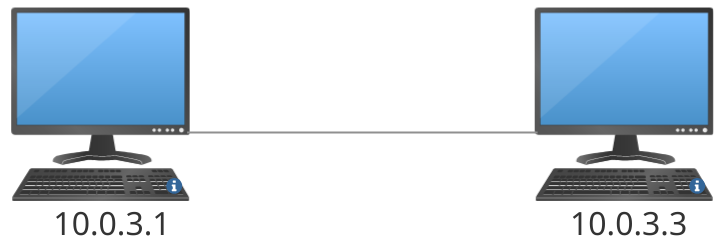
\includegraphics[width=0.30\linewidth]{network-topology.png}
    \caption{Network Topology}
    \label{fig:enter-label}
\end{figure}
\begin{table}[H]
  \begin{center}
    \begin{tabular}{|l|l|l|}
      \hline
      \textbf{Host name} & \textbf{IP address} & Role \\
      \hline
      H1 & 10.0.3.1/25 & Server \\
      \hline
      H3 & 10.0.3.3/25  & Client \\
      \hline
    \end{tabular}
  \end{center}
  \caption{Net hosts}\label{tab:net-hosts}
\end{table}


\section{Experiment Setup}

\begin{figure}[H]
    \centering
    \begin{subfigure}[b]{0.40\textwidth}
        \centering
        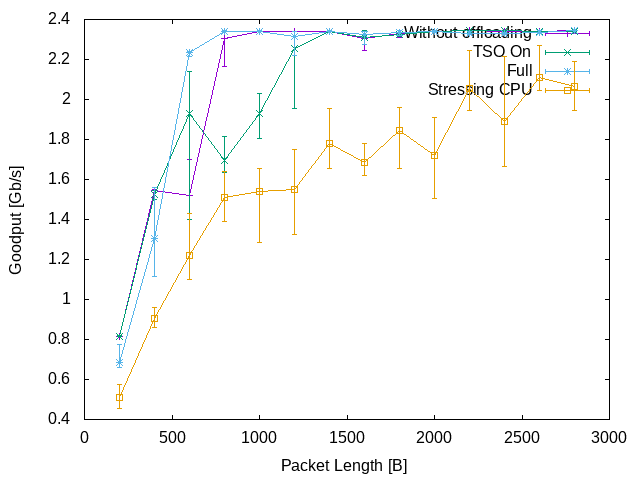
\includegraphics[width=\textwidth]{iperf/throughput.png}
        \caption{Good-put against Payload Length}
        \label{fig:good}
    \end{subfigure}
    \hfill
        \begin{subfigure}[b]{0.40\textwidth}
        \centering
        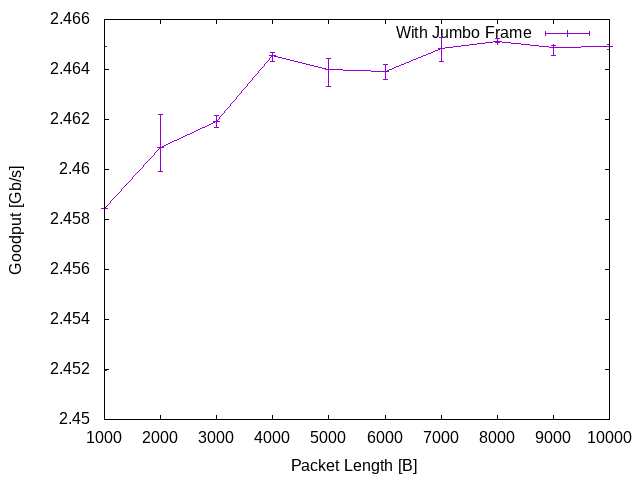
\includegraphics[width=\textwidth]{iperf/throughput_j.png}
        \caption{Good-put with Jumbo Frames enabled}
        \label{fig:good-j}
    \end{subfigure}
    \hfill
    \begin{subfigure}[b]{0.40\textwidth}
        \centering
        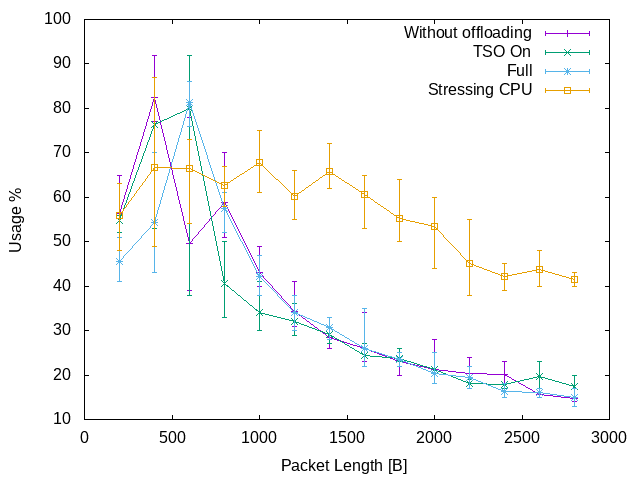
\includegraphics[width=\textwidth]{iperf/cpu.png}
        \caption{CPU Usage \%}
        \label{fig:cpu}
    \end{subfigure}
    \hfill
    \begin{subfigure}[b]{0.40\textwidth}
        \centering
        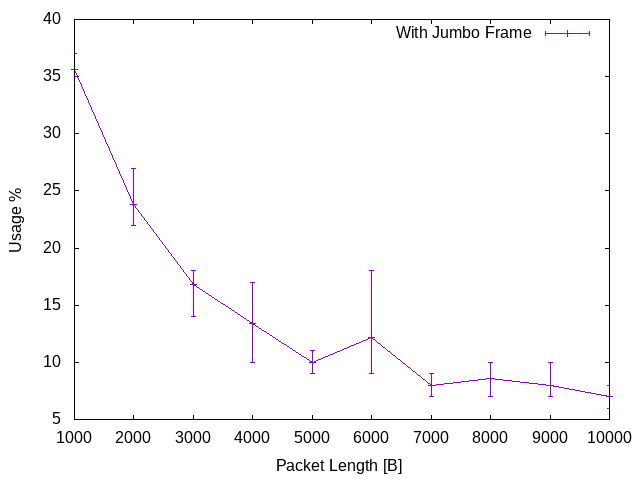
\includegraphics[width=\textwidth]{iperf/cpu_j.png}
        \caption{CPU Usage \% with Jumbo}
        \label{fig:cpu-j}
    \end{subfigure}

    \caption{\texttt{iperf3} capture (On the Sender)}
\end{figure}

\begin{figure}[H]
    \centering
    \begin{subfigure}[b]{0.40\textwidth}
        \centering
        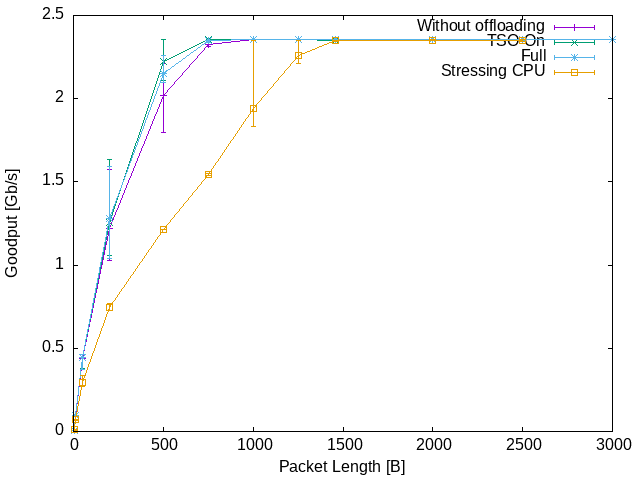
\includegraphics[width=\textwidth]{nttcp/throughput.png}
        \caption{Good-put against Payload Length}
        \label{fig:n-good}
    \end{subfigure}
    \hfill
        \begin{subfigure}[b]{0.40\textwidth}
        \centering
        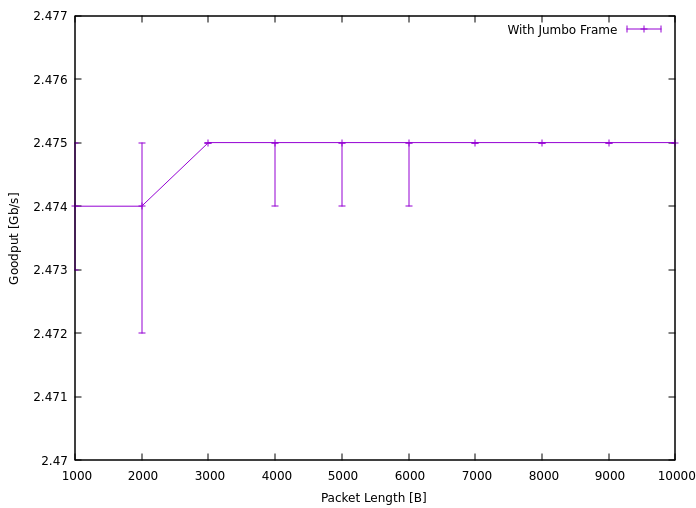
\includegraphics[width=\textwidth]{nttcp/throughput_j.png}
        \caption{Good-put with Jumbo Frames enabled}
        \label{fig:n-good-j}
    \end{subfigure}
    \hfill
    \begin{subfigure}[b]{0.40\textwidth}
        \centering
        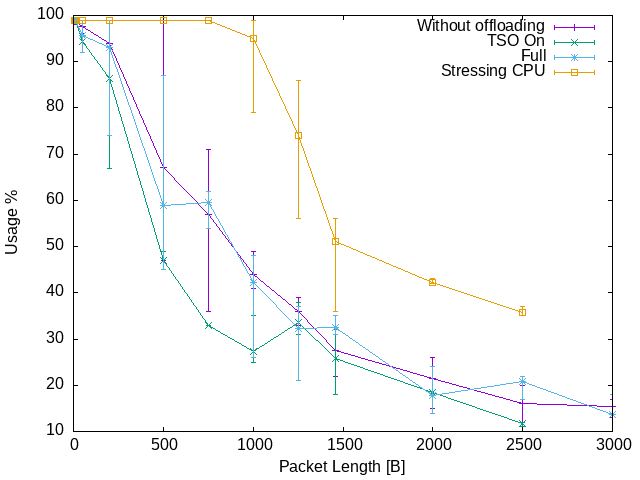
\includegraphics[width=\textwidth]{nttcp/cpu.png}
        \caption{CPU Usage \%}
        \label{fig:n-cpu}
    \end{subfigure}
    \hfill
    \begin{subfigure}[b]{0.40\textwidth}
        \centering
        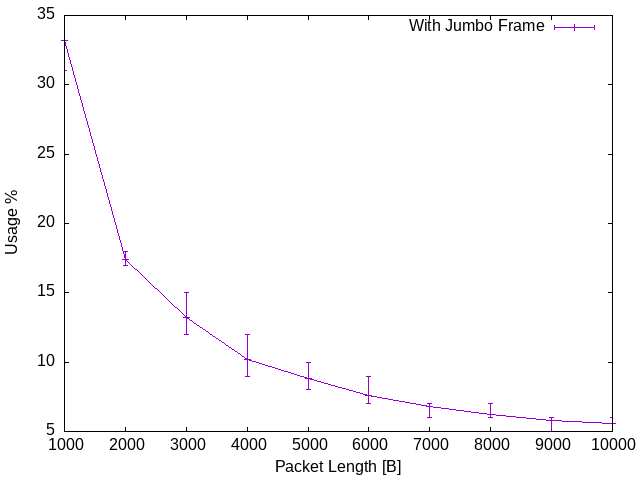
\includegraphics[width=\textwidth]{nttcp/cpu_j.png}
        \caption{CPU Usage \% with Jumbo}
        \label{fig:n-cpu-j}
    \end{subfigure}

    \caption{\texttt{nttcp} capture (On the Sender)}
\end{figure}

We performed a series of experiments to test how the different sizes of packet length impacted the \textbf{Good-put} in a TCP communication; this was done in conjunction with the offloading capabilities of the Network Card used for this experiment, which was \textit{Realtek 2.5Gb}. We conducted 5 kinds of experiment with each program to do \textbf{speed tests}: \texttt{iperf3} and \texttt{nttcp}. The various configurations were all tested on the Sender (sends data), on which the measurements were taken:
\begin{itemize}
    \item \textbf{No Offloading Enabled.}
    \item \textbf{TSO Offloading Enabled.}
    \item \textbf{Every Offloading Capability Enabled (RX/TX + SG + TSO + GSO + GRO).}
    \item \textbf{Every Offloading Capability Enabled with the System Under Stress.}
    \item \textbf{Every Offloading Capability Enabled with the Jumbo Frame Enabled.}
\end{itemize}

\subsection{Comparison between \texttt{nttcp} and \texttt{iperf3}}

After performing various tests and plotting the data retrieved, using both \texttt{iperf3} and \texttt{nttcp}, we noticed that the graphical trends generally resemble each other, but with some noticeable differences:
\begin{itemize}
    \item by looking at the \textbf{CPU usage \%} graphs, it can be noted that the CPU usage is averagely much higher using \texttt{nttcp}; in fact, we can see that, when the packet size is low, the CPU's busyness is over 90\%, especially in the \textbf{Stressing CPU} case. This could lead to think that \texttt{nttcp} implements a rower \textit{sending-loop}, while \texttt{iperf3} provides a more sophisticated one, with some level of optimization in the way it sends the buffers to the server.
    \item by looking at the \textbf{Good-put against Payload Length} graphs, it is possible to see that the graphical progress is more stable when using \texttt{nttcp}: the boundaries are clearer and it actually takes the shape of a monotonic increasing curve, which is as expected when increasing the packet size; it cannot be said the same for the experiment with \texttt{iperf3}, as it can be observed that the curves have many more oscillations than the ones of \texttt{nttcp} and the boundaries are more uncertain.
    \item by looking again at the \textbf{Good-put against Payload Length} graphs, using \texttt{nttcp}, the good-put establishes itself at around 2.3 Gb/s with block size from about 750 bytes on (with the exception of the \textbf{Stressing CPU} case, whose block size to get the same behavior is from about 1500 bytes on). On the other hand, using \texttt{iperf3}, this trend is replicated only when all offloading capabilities are disabled or enabled; if the TSO is the only offloading capability enabled, \texttt{iperf3} struggles more to reach the saturation point and, in case of \textbf{Stressing CPU}, a stability in the good-put is actually never reached for the duration of the experiment, even for block size over 2500 bytes.
    \item by looking at the \textbf{Good-put with Jumbo Frames enabled} graphs, it can be seen that \texttt{nttcp} reaches the saturation with packet length equal to 3000 bytes, while \texttt{iperf3} touches the saturation point at 4000 bytes packet length and then struggles to maintain its stability.
\end{itemize}

\subsection{Theoretical Limits of the Good-put} 
We can now take a rough calculation of what is the \textbf{efficiency} of this exchange of TCP messages. We can estimate, for the maximum efficiency, that TCP is exchanging data using the MSS and, by taking into account the additional overhead, we can calculate the efficiency $\eta_{TCP}$.
\[
\eta_{TCP} = \frac{1448_{MSS}}{1448_{MSS} + 32_{TCP_H} + 20_{IP_H} + 38_{ETH_H}} = 94\%
\]
If we compute the theoretical maximum \textbf{good-put} on the $2.5 Gb/s$ network card we get: $\eta_{TCP} \cdot 2.5 Gb/s = 2.35 Gb/s$; as a matter of facts, we get as the maximum value of the \textbf{Good-put} from \texttt{nttcp} and \texttt{iperf3} at about $2.35 Gb/s$ and $2.34 Gb/s$ respectively, for which, in both cases, all the offloading capabilities were enabled.

If we enable \textbf{jumbo frames} on the network card, we can have a MTU of 9000 Bytes. By doing so, we do not increase the speed of the network card but we increase the \textbf{efficiency}.
\[
\eta_{TCP,Jumbo} = \frac{8948_{MSS}}{8948_{MSS} + 32_{TCP_H} + 20_{IP_H} + 38_{ETH_H}} = 99\%
\]
\begin{wrapfigure}{r}
    \centering
    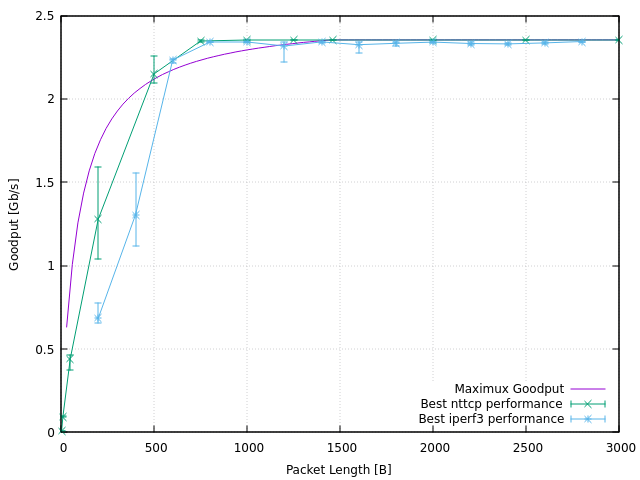
\includegraphics[width=0.40\textwidth]{maximum-goodput.png}
    \caption{Maximum Good-put (No Jumbo)}
    \label{fig:maximum-goodput}
\end{wrapfigure}
We can compute the maximum theoretical \textbf{Good-put} with \textbf{Jumbo Frames} enabled, which is $\eta_{TCP,Jumbo} \cdot 2.5 Gb/s = 2.476 Gb/s$. In the graphs, we observe that, by increasing the packet size up to 10000 bytes, we get a good-put of about $2.475 Gb/s$ and  $2.465 Gb/s$ for \texttt{nttcp} and \texttt{iperf3} respectively, for which, in both cases, all the offloading capabilities were enabled.


\subsection{Impact of the block size on the Good-put}
The first thing we can observe from the graph is, in every analyzed case, that an increase in block size leads to an improvement in \verb|Good-put|, but further considerations must be done.

As shown in figure~\ref{fig:maximum-goodput}, it's possible to see the two best scenarios for both \texttt{nttcp} and \texttt{iperf3} plotted against the theoretical maximum good-put curve and what immediately catches the eye is that the actual curves are significantly different from the theoretical curve.
For small \verb|Block size|, in fact, we have a sub-optimal \verb|Good-put|; an explanation for this phenomenon can be extrapolated by looking at the \textbf{CPU usage \%}: with small blocks we can notice that the CPU usage is very high, due to \texttt{iperf3} and \texttt{nttcp} creating in loop many small buffers and then invoking the system call \texttt{write()} to send the data through the \textbf{socket}. The majority of the time is spent creating these small buffers and invoking a \textbf{system call}, the latter being a particularly complex operation from a computational point of view.

At around 800 bytes in \verb|Block size|, we observe an even stranger phenomenon: the real \verb|Good-put| curve surpasses the \verb|theoretical maximum good-put|, which is supposed to be a non surmountable limit. In reality, using \textbf{Wireshark}, we observed that for most of the packets' payload length was bigger than the \verb|Block size| set in the running application for \verb|block size| smaller than 1448 bytes.
Due to the way TCP segmentation is implemented, the kernel (or the Network Interface when TSO is ON) groups multiple blocks to achieve better efficiency, resulting in increased \verb|Good-put|, while our theoretical curve doesn't address this behavior. Not knowing how the kernel is implemented, we can theorize as another plausible reason for this behavior that, when the application make a \texttt{write()} system call on a socket, the kernel will maintain an \textbf{inner buffer} that will dump on the socket only when it is not busy; as a consequence, other calls to the \texttt{write()} system call might add more data to that specific buffer before it is actually passed to the underlying layer. 
As a side note, this behavior is also noticeable in the figure~\ref{fig:n-good-j}, where the \textbf{good-put} already starts saturating at 3000 bytes, this should not be possible, in fact that Good-put value can only be achieved at MSS, but as said above, the Kernel performs some optimizations.

From this point onward, as the \verb|Block size| increase, the actual curves consistently tend more closely towards the theoretical curve because the TCP segmentation is limited by the MTU size.

\subsection{CPU time for the tests}
We used, as a measure of \verb|CPU-load|, the percentage of CPU used during the processing of an experiment; in order to retrieve this value, we used \verb|/usr/bin/time| followed by the \texttt{nttcp/iperf3} command. One detail that catches the eye is that the CPU usage of \texttt{nttcp} is always higher than the CPU usage of \texttt{iperf3}; this could be due to the fact that \texttt{iperf3} has a \texttt{pselect()} system call between the \texttt{write()} system calls (we observed that using \texttt{strace}). As stated in the \href{https://linux.die.net/man/2/pselect}{Documentation}, this system call monitors the state of a File Descriptor, and returns when its state is ready for an operation to be performed on; in our case, the \texttt{pselect()} waits for the socket to be ready, and then the process writes on it, allowing to reduce the workload on the CPU.

\section{Analysis of the offloading capabilities}
\subsection{Driver's offloading capabilities}
The driver offers a variety of offloading capabilities. These are:
\begin{itemize}
    \item \textbf{Receiving/Transmission Offloading (RX/TX)}: this capability allows the NIC of the receiver/transmitter to perform the validation of the checksum field for the \texttt{TCP} header, while the \texttt{IP} checksum is always validated through software, because, when it is built, it is already in cache, so it is not expensive to sum it, as stated in the \href{https://www.kernel.org/doc/html/next/networking/checksum-offloads.html}{Linux Documentation}.
    \item \textbf{TCP Segmentation Offloading (TSO)}: this capability allows the usage of the NIC card to segment large chunks of data into smaller TCP segments, also adding a TCP, an IP and an Ethernet header, in order to reduce the CPU overhead, this can be enabled only if RX/TX and Scatter Gather are enabled. If this capability is disabled, then the CPU has the burden to segment the data before the individual packets will be sent.
    \item \textbf{Large Receive Offload (LRO)}: this capability allows to reassemble small packets into larger buffers as they are received, reducing the number that the CPU has to process.
    \item \textbf{Scatter-gather (SG)}: this capability allows to pass around small buffers that make up for a big logical one, instead of passing directly the large packet; this allows a quicker and more efficient data processing .
    \item \textbf{Generic Segmentation/Receive Offloading (GSO/GRO)}: this is an alternative to the solution proposed by the TSO capability, which means to handle, through a specific software implementation, the segmentation when the NIC is not capable of doing so. It allows upper layer applications to process large packets and the segmentation is delayed as much as possible, reducing per-packet overhead.
\end{itemize}

\subsection{Impact of the offloading capabilities}
Observing the graphs \ref{fig:cpu} and \ref{fig:n-cpu}, we can perceive how different network interface offloading settings can generate small but not unnoticeable changes in the CPU load. 


\subsubsection{Difference between Nttcp and Iperf3}
First of all we observe slightly different behavior between the \verb|Iperf3| graphs and the \verb|Nttcp| graphs. 
Starting from Nttcp, we can notice a way more aggressive implementation: the CPU load when payload is short reaches nearly 100\% without any stress from outside sources. This overhead seems to be caused by an uncontrolled usage of the syscall \verb|write| and the following context switch between user and kernel mode: in fact, this overhead seems to become increasingly negligible as the length of the packets grows and the biggest part of the CPU load becomes the generation of the payload and with it the differences with \verb|Iperf3| decrease.

By using \verb|strace|, we spot that in \verb|Iperf3| the calls to the \verb|write| system-call are interleaved with calls to the \verb|pselect|, another system call used to monitor file descriptor and the possible action that can be performed to the corresponding file to avoid CPU waste. 

Even if not relevant to this experiment, by using \verb|strace| we also observe that the reason why the \verb|nttcp| receiver has more system calls than the sender is the presence of a continuous call to a non-blocking \verb|read| syscall, without first checking that the socket isn't empty.

\subsubsection{Offloading configuration differences}
Once the differences between the two applications are overcome, we can focus on the differences between the different configuration we can adopt on the Network Interface.
Starting by disabling all the offloading, we can observe that the curve representing this scenario is, in average, above the other curves of the \textit{non-stressed cluster}. This curve differs significantly from the others between \verb|Block size| of 500 and 1200 bytes, where there's more than a 20\% load difference with the \verb|TSO on curve|. When the \verb|Block size| is big, the overhead caused by the TCP/IP stack's headers to add becomes negligible and with it the differences with the other curves.

In one of the other test we enabled all the offloading and in the other one we  only enabled the \verb|TSO| and found out that the latter, even if counter-intuitively, has slightly better performance. This could be caused by the fact that we only use TCP in this experience and a more generic set of offloads isn't needed, causing a loss of performance. 

\subsection{Analysis with Jumbo frames}
This experiment aims to observe the behavior of the network and its properties in terms of \verb|Good-put| and \verb|CPU-load| when jumbo frames and all offloads are enabled.

\subsubsection{Good-put with Jumbo frame}
The first thing we can observe is the greater \verb|Good-put| that nearly saturates the capacity of the channel, even with short length payload, with a value of  $2.458 Gb/s$ (in the \texttt{iperf3} case), greater than the maximum \verb|Good-put| reached with a normal MTU of 1500. This is a direct consequence of a better \verb|efficiency| compared to a standard MTU: the \verb|TSO and GSO| collect a lot more data before adding the packet's header, consequentially increasing the \verb|Good-put|. The \verb|Good-put| continues to slightly increase in a directly proportional manner to the \verb|Block size|. In  Figure~\ref{fig:jumbo-comparison}, we can see the different graphs compared to each other (when all the Offloading Capabilities are enabled): it's noticeable that, even when the packet size is set at around 1000 Bytes, the efficiency of the Jumbo packets is much greater then the one without them. If the kernel or the NIC decides to group more data, when the process passes its blocks to the underlying layers, then it will probably send them in packets a lot larger than 1000 Bytes.

\begin{wrapfigure}{r}
    \centering
    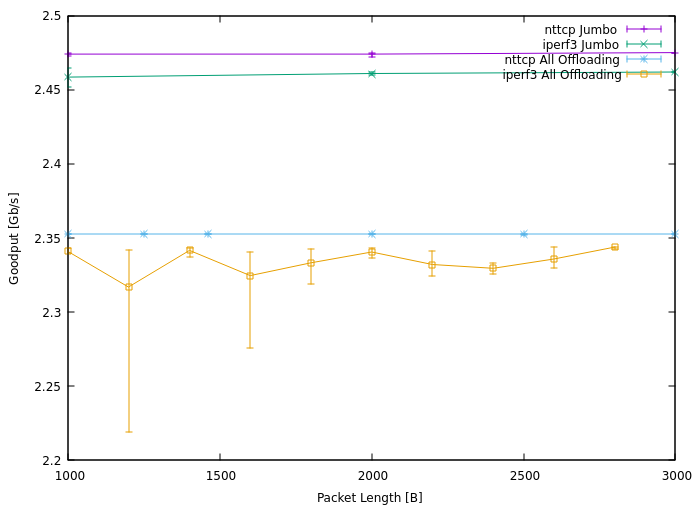
\includegraphics[width=0.40\textwidth]{jumbo-comparison.png}
    \caption{Comparing Jumbo to Non-Jumbo Tests}
    \label{fig:jumbo-comparison}
\end{wrapfigure}

\subsubsection{CPU load with Jumbo frames}
The \verb|CPU-load| in this experience is exactly the same as the corresponding one (Full offload) with a 1500 bytes MTU. The only cause of the \verb|CPU-load| is the generation of the payload, that has no differences in the two scenarios, while all the TCP/IP stack headers are managed by the Network Interface. We would probably observe a decrease in the \verb|CPU-load| with the Network Interface offloading disabled because the headers would be built at the expense of CPU resources and less headers are needed with a bigger MTU. 

In this experiment we went way further with the \verb|Block size| and, as expected, the \verb|CPU-load| continues to decrease in an inversely proportional manner relative to it.

\section{Performances with busy CPU}
We run \verb|stress| application to test the network behavior when the transmitter is overloaded. The first thing we observe is a significant loss in term of \verb|Good-put| and also a significant increase in the CPU usage of both the application.

\subsection{CPU-load}
The most relevant thing we can observe is the increase in the CPU-load: the scheduler need to context switch a lot more between the applications when the system is stressed, causing a significant increase in the CPU usage of our applications.
While, apparently, both \verb|Nttcp| and \verb|iperf| show the same general behavior, upon closer inspection differences can be noticed. Contrary to what was seen earlier \texttt{nttcp} has a lower system load compared to \texttt{iperf3} (beside for small block size where is still 100\%). Paradoxically, this could be due to the more aggressive approach nttcp uses: by leaving to the scheduler less opportunities to switch to another thread, the context-switch overhead decreases.
\subsection{Good-put}
What we have just seen is also reflected in the \verb|Good-put|: while nttcp, even if at higher block sizes, is able to saturate the channel capacity, iperf3 fails to do so at any block size. In any case, the general trend is towards a lower good-put compared to a non-overloaded system.

\subsection{Test reliability consideration}
The result we obtained are also not very reliable because iperf3 sends data until 10 seconds are passed while nttcp sends a constant quantity of bytes. In an overloaded system the quantity of bytes sent in a fixed quantity of time and the time needed to send a fixed quantity of bytes is a lot more unpredictable, causing a greater variance over the experiment.

\pagebreak
\section{Appendix}
\subsection{Script to generate iperf3 graphs}
\begin{lstlisting}[language=python]
#!/bin/python3

import os
import json
import argparse
from subprocess import Popen, PIPE

parser = argparse.ArgumentParser()
parser.add_argument('-r', '--retrans', action='store', type=int, default=5, help='number of retransmissions')
parser.add_argument('-s', '--step', action='store', type=int, default=300, help='number of steps to reach 3000 bytes')
parser.add_argument('--interface', action='store', type=str, default='eth0', help='interface to modify the offloading')
parser.add_argument('-S', '--server', action='store', type=str, default='10.0.3.1', help='server to connect')
parser.add_argument('-i', '--interactive', action='store_true', help='run gnuplot in interactive mode')
parser.add_argument('-t', '--test', choices=['tso_on', 'full', 'no_off', 'stressed', 'jumbo', 'jumbo_long'], nargs='+', help='test for different modes')
parser.add_argument('-k', '--keepold', action='store_true', help='set if you want to don\'t override old files')
parser.add_argument('-j', '--jumbo', action='store_true', help='do the jumbo test')
args = parser.parse_args()

RETRANS = args.retrans
INTERFACE = args.interface
STEP = args.step
SERVER = args.server
INTERACTIVE = args.interactive
KEEP_OLD = args.keepold
JUMBO = args.jumbo
TEST = args.test if args.test is not None else []

def get_receiver(proc):
    out = proc.stdout.read().decode()
    out = json.loads(out)
    return out["end"]["streams"][0]["receiver"]

def get_cpu(proc):
    out = proc.stderr.read().decode()
    return int(out.replace("%", ""))

def show_res(receiver):
    print(receiver)
    print(receiver["bytes"])

def write_out(output, packet_len, bit_s, bit_min, bit_max, cpu, cpu_min, cpu_max, out_name):
    print(f"len:{packet_len} bit_s:{bit_s} min:{bit_min} max:{bit_max} cpu:{cpu} cpu_min:{cpu_min} cpu_max:{cpu_max}")
    line = f"{packet_len} {bit_s} {bit_min} {bit_max} {cpu} {cpu_min} {cpu_max}\n"
    output.write(line)
    #os.system(f"echo {packet_len} {bit_s} {bit_min} {bit_max} {cpu} {cpu_min} {cpu_max}>> {out_name}")

def run_test(out_name, jumbo = False):
    stop = 3000 if not jumbo else 10001

    with open(out_name, "w") as output:
        for packet_len in range(STEP, stop, STEP):
            bit_s = []
            cpu_t = []
            for _ in range(RETRANS):
                with Popen(["/usr/bin/time", "-f", "%P", "iperf3", "-J", "-l", str(packet_len), "-c", SERVER], stdout=PIPE, stderr=PIPE) as proc:
                    # Convert them in Gb/s
                    bit_s.append(get_receiver(proc)["bits_per_second"] / 1e9)
                    cpu_t.append(get_cpu(proc))

            bit_min = min(bit_s)
            bit_max = max(bit_s)
            bit_s = sum(bit_s) / RETRANS

            cpu_min = min(cpu_t)
            cpu_max = max(cpu_t)
            cpu = sum(cpu_t) / RETRANS

            write_out(output, packet_len, bit_s, bit_min, bit_max, cpu, cpu_min, cpu_max, out_name)


if 'tso_on' in TEST:
    print('tso on')
    os.system(f"sudo ethtool -K {INTERFACE} rx on tx on sg on tso on gso off gro off")
    run_test('tso_on')


if 'full' in TEST:
    print("full")
    os.system(f"sudo ethtool -K {INTERFACE} rx on tx on sg on tso on gso on gro on")
    run_test("full")


if 'no_off' in TEST:
    print("no offloading")
    os.system(f"sudo ethtool -K {INTERFACE} rx off tx off sg off tso on gso off gro off")
    run_test('no_off')
        

if 'stressed' in TEST:
    print("cpu stressed")
    os.system(f"sudo ethtool -K {INTERFACE} rx on tx on sg on tso on gso on gro on")
    proc = Popen("stress --cpu 8 --io 4 --vm 2 --vm-bytes 128M --timeout 1000s".split())
    run_test("stressed")
    proc.kill()

if 'jumbo' in TEST:
    print('jumbo frame')
    os.system(f"sudo ethtool -K {INTERFACE} rx on tx on sg on tso on gso on gro on")
    os.system(f"sudo ifconfig {INTERFACE} mtu 9000")
    run_test('jumbo', True)
    os.system(f"sudo ifconfig {INTERFACE} mtu 1500")

# Gnuplot section
persist = '-persist' if INTERACTIVE else ''

def output(out): 
    return '' if INTERACTIVE else '''set term png
set output "{0}"
'''.format(out)

gnuplot_cmd = '''gnuplot {0} <<EOF
{1}
set xlabel "Packet Length [B]"
set ylabel "{2}"
plot "no_off" using 1:{3} with errorline title "Without offloading", \
    "tso_on" using 1:{3} with errorline title "TSO On", \
    "full" using 1:{3} with errorline title "Full", \
    "stressed" using 1:{3} with errorline title "Stressing CPU"
EOF
'''

# Goodput
os.system(gnuplot_cmd.format(persist, output("throughput.png"), "Goodput [Gb/s]", "2:3:4"))

# CPU
os.system(gnuplot_cmd.format(persist, output("cpu.png"), "Usage %", "5:6:7"))

# JUMBO
gnuplot_cmd = '''gnuplot {0} <<EOF
{1}
set xlabel "Packet Length [B]"
set ylabel "{2}"
plot "jumbo" using 1:{3} with errorline title "With Jumbo Frame"
EOF
'''

# Goodput
os.system(gnuplot_cmd.format(persist, output("throughput_j.png"), "Goodput [Gb/s]", "2:3:4"))

# CPU
os.system(gnuplot_cmd.format(persist, output("cpu_j.png"), "Usage %", "5:6:7"))
\end{lstlisting}

\subsection{Script to generate nttcp graphs}

\begin{lstlisting}[language=bash]
#!/bin/sh
H1=10.0.3.1


/usr/bin/time -f "%P" nttcp -n $1 -l $2 $H1 > data$2.dat 2> cpu$2.dat

Cpu=$(cat cpu$2.dat | tr -d "%")
Tx=$(cat data$2.dat | tail -n 2 | head -n 1 | tr -s " ")
Rx=$(cat data$2.dat | tail -n 1 | head -n 1 | tr -s " ")
Gtx=$(echo $Tx | cut -d " " -f5)
Grx=$(echo $Rx | cut -d " " -f5)

echo $1 $2 >> megalog.log
echo $Tx >> megalog.log
echo $Rx >> megalog.log
echo "" >> megalog.log

echo $Gtx $Grx $Cpu
\end{lstlisting}
\begin{lstlisting}[language=python]
#!/bin/python3

import os
import json
import argparse
from subprocess import Popen, PIPE

parser = argparse.ArgumentParser()
parser.add_argument('-r', '--retrans', action='store', type=int, default=5, help='number of retransmissions')
parser.add_argument('-s', '--step', action='store', type=int, default=300, help='number of steps to reach 3000 bytes')
parser.add_argument('--interface', action='store', type=str, default='eth0', help='interface to modify the offloading')
parser.add_argument('-S', '--server', action='store', type=str, default='10.0.3.1', help='server to connect')
parser.add_argument('-i', '--interactive', action='store_true', help='run gnuplot in interactive mode')
parser.add_argument('-t', '--test', choices=['tso_on', 'full', 'no_off', 'stressed', 'jumbo', 'jumbo_long'], nargs='+', help='test for different modes')
parser.add_argument('-k', '--keepold', action='store_true', help='set if you want to don\'t override old files')
parser.add_argument('-j', '--jumbo', action='store_true', help='do the jumbo test')
args = parser.parse_args()

RETRANS = args.retrans
INTERFACE = args.interface
STEP = args.step
SERVER = args.server
INTERACTIVE = args.interactive
KEEP_OLD = args.keepold
JUMBO = args.jumbo
TEST = args.test if args.test is not None else []


ls = [1, 3, 10, 50, 100, 200, 500, 750, 1000, 1250, 1448, 2000, 2500, 3000]
ns = [14000000, 13000000, 13000000, 12000000, 11000000, 7000000, 5000000, 4000000, 3000000, 2500000, 2000000, 1500000]

def get_receiver(proc):
    out = proc.stdout.read().decode()
    out = out.split()
    return float(out[1]), float(out[2])

def get_cpu(proc):
    out = proc.stderr.read().decode()
    return int(out.replace("%", ""))

def show_res(receiver):
    print(receiver)
    print(receiver["bytes"])

def write_out(output, packet_len, bit_s, bit_min, bit_max, cpu, cpu_min, cpu_max, out_name):
    print(f"len:{packet_len} bit_s:{bit_s} min:{bit_min} max:{bit_max} cpu:{cpu} cpu_min:{cpu_min} cpu_max:{cpu_max}")
    line = f"{packet_len} {bit_s} {bit_min} {bit_max} {cpu} {cpu_min} {cpu_max}\n"
    output.write(line)
    #os.system(f"echo {packet_len} {bit_s} {bit_min} {bit_max} {cpu} {cpu_min} {cpu_max}>> {out_name}")

def run_test(out_name, jumbo = False):
    stop = 3000 if not jumbo else 10001

    with open(out_name, "w") as output:
        for n, l in zip(ns, ls):
            bit_s = []
            cpu_t = []
            for _ in range(RETRANS):
                with Popen(f'./script.sh {n} {l}'.split(), stdout=PIPE, stderr=PIPE) as proc:
                    # Convert them in Gb/s
                    r = get_receiver(proc)
                    print(r)
                    bit_s.append(r[0] / 1e3)
                    cpu_t.append(r[1])

            bit_min = min(bit_s)
            bit_max = max(bit_s)
            bit_s = sum(bit_s) / RETRANS

            cpu_min = min(cpu_t)
            cpu_max = max(cpu_t)
            cpu = sum(cpu_t) / RETRANS

            write_out(output, packet_len, bit_s, bit_min, bit_max, cpu, cpu_min, cpu_max, out_name)


if 'tso_on' in TEST:
    print('tso on')
    os.system(f"sudo ethtool -K {INTERFACE} rx on tx on sg on tso on gso off gro off")
    run_test('tso_on')


if 'full' in TEST:
    print("full")
    os.system(f"sudo ethtool -K {INTERFACE} rx on tx on sg on tso on gso on gro on")
    run_test("full")


if 'no_off' in TEST:
    print("no offloading")
    os.system(f"sudo ethtool -K {INTERFACE} rx off tx off sg off tso on gso off gro off")
    run_test('no_off')
        

if 'stressed' in TEST:
    print("cpu stressed")
    os.system(f"sudo ethtool -K {INTERFACE} rx on tx on sg on tso on gso on gro on")
    proc = Popen("stress --cpu 8 --io 4 --vm 2 --vm-bytes 128M --timeout 1000s".split())
    run_test("stressed")
    proc.kill()

if 'jumbo' in TEST:
    print('jumbo frame')
    os.system(f"sudo ethtool -K {INTERFACE} rx on tx on sg on tso on gso on gro on")
    os.system(f"sudo ifconfig {INTERFACE} mtu 9000")
    run_test('jumbo', True)
    os.system(f"sudo ifconfig {INTERFACE} mtu 1500")

# Gnuplot section
persist = '-persist' if INTERACTIVE else ''

def output(out): 
    return '' if INTERACTIVE else '''set term png
set output "{0}"
'''.format(out)

gnuplot_cmd = '''gnuplot {0} <<EOF
{1}
set xlabel "Packet Length [B]"
set ylabel "{2}"
plot "no_off" using 1:{3} with errorline title "Without offloading", \
    "tso_on" using 1:{3} with errorline title "TSO On", \
    "full" using 1:{3} with errorline title "Full", \
    "stressed" using 1:{3} with errorline title "Stressing CPU"
EOF
'''

# Goodput
os.system(gnuplot_cmd.format(persist, output("throughput.png"), "Goodput [Gb/s]", "2:3:4"))

# CPU
os.system(gnuplot_cmd.format(persist, output("cpu.png"), "Usage %", "5:6:7"))

# JUMBO
gnuplot_cmd = '''gnuplot {0} <<EOF
{1}
set xlabel "Packet Length [B]"
set ylabel "{2}"
plot "jumbo" using 1:{3} with errorline title "With Jumbo Frame"
EOF
'''

# Goodput
os.system(gnuplot_cmd.format(persist, output("throughput_j.png"), "Goodput [Gb/s]", "2:3:4"))

# CPU
os.system(gnuplot_cmd.format(persist, output("cpu_j.png"), "Usage %", "5:6:7"))

\end{lstlisting}

\end{document}